%*******************************************************
% Annexe — Semi-conducteurs, IA générative et couplage énergétique
% Avril 2026 — Document de travail
%*******************************************************

\chapter{Semi-conducteurs, IA générative et couplage énergétique}\label{ch:annexe-genai}

\noindent\emph{Cette annexe fournit le matériau empirique contemporain que l'analyse économique du chapitre~2 mobilise dans ses tests. Elle prolonge le travail d'induction analytique du chapitre~1 en examinant le cas de l'industrie des semi-conducteurs et de l'intelligence artificielle générative~--- non pas pour appliquer mécaniquement une grille à dix entrées, mais pour repérer où les mécanismes identifiés historiquement se confirment, où ils changent de forme, et surtout, où le couplage entre infrastructure informationnelle et substrat énergétique cesse d'être négligeable. Le diagnostic est exploratoire~: il identifie des invariances, des accélérations et des inversions, mais ne les teste pas.}

\bigskip

\section{L'économie des semi-conducteurs~: une course aux rendements d'échelle sous contrainte de coûts croissants}

L'industrie des semi-conducteurs repose sur un équilibre dynamique entre deux forces. D'un côté, la densité de transistors par circuit intégré a doublé approximativement tous les dix-huit mois à coût unitaire réduit pendant quatre décennies~--- c'est l'observation formulée par \textcite{moore_cramming_1965} et transformée depuis en feuille de route industrielle. Moore lui-même a insisté sur la nature économique de sa projection~: la loi ne décrit pas une contrainte physique mais le nombre de composants le plus rentable pour un contexte industriel donné\footnote{Dans une conférence tardive, Moore résumait~: \og \emph{Moore's law is really about economics}\fg{} (cité dans \emph{The Chip Letter}, 2025).}. Cette dynamique n'est pas terminée~--- TSMC grave du 3~nm en production, vise le 2~nm en 2025, et les feuilles de route d'ASML projettent jusqu'à l'angström en 2036~--- mais ses conditions ont changé. Le rythme a ralenti (six ans pour passer de 7 à 2~nm, contre dix-huit mois par nœud dans les années~1990). Le coût unitaire par transistor ne baisse plus sous le seuil des 10~nm \parencite{pirson_environmental_2022}. Et les gains passent désormais par des innovations architecturales~--- empilement 3D (CoWoS), transistors Gate-All-Around, chiplets~--- autant que par la miniaturisation proprement dite. Ce qui n'a pas changé, c'est la fonction performative de la loi~: elle reste le baromètre de la capacité de l'industrie à mobiliser des investissements à grande échelle. De l'autre côté, le coût de construction d'une fonderie avancée double tous les quatre ans~--- c'est la loi de Rock, moins connue mais tout aussi structurante \parencite{ross_moores_1995}. Le coût moyen d'une fonderie est passé de 31~millions de dollars dans les années~1980 à 13,4~milliards pour la Fab~15 de TSMC et 25~milliards pour la fonderie Samsung Taylor\footnote{Sources~: VLSI Research~; McKinsey~; rapports annuels TSMC.}. Le progrès technologique n'est donc rentable que s'il s'accompagne d'économies d'échelle suffisantes pour que la baisse du coût unitaire compense la hausse du coût de production. \textcite{gruber_semiconductor_1996} a montré que les cycles baissiers de l'industrie se traduisent par une compression des marges~: les fabricants doivent choisir entre rentabilité et parts de marché, et les parts de marché l'emportent parce qu'elles conditionnent les économies d'échelle futures.

Ce mécanisme a une conséquence structurelle~: la puissance de calcul mise sur le marché chaque année doit être \emph{consommée} pour justifier les investissements de la génération suivante. Il en résulte une boucle de création de demande~: Moore fournit la trajectoire technique, Rock crée la contrainte d'investissement, et la coordination entre fabricants de composants et éditeurs de logiciels assure l'absorption. L'empreinte environnementale croissante est une externalité de cette boucle, pas une rétroaction~: elle n'en modifie pas la dynamique. Pendant quatre décennies, cette absorption a été assurée par l'alliance entre fabricants de composants et éditeurs de logiciels. L'alliance Windows-Intel (dite Wintel) illustre le mécanisme~: chaque génération de processeur Intel était accompagnée d'une version de Windows suffisamment gourmande en ressources pour saturer les nouvelles capacités \parencite{gilder_coming_1995}. L'espace ouvert par les gains de puissance servait de soupape~: les logiciels devenaient moins efficaces mais plus fonctionnels, sans que cette inefficacité n'ait de coût marginal pour l'éditeur\footnote{\textcite{schaller_origin_1996} documente la dynamique côté logiciel~: le nombre de lignes de code de Word passe de 27\,000 en 1982 à 2~millions en 1995.}.

\begin{figure}[htbp]
\centering
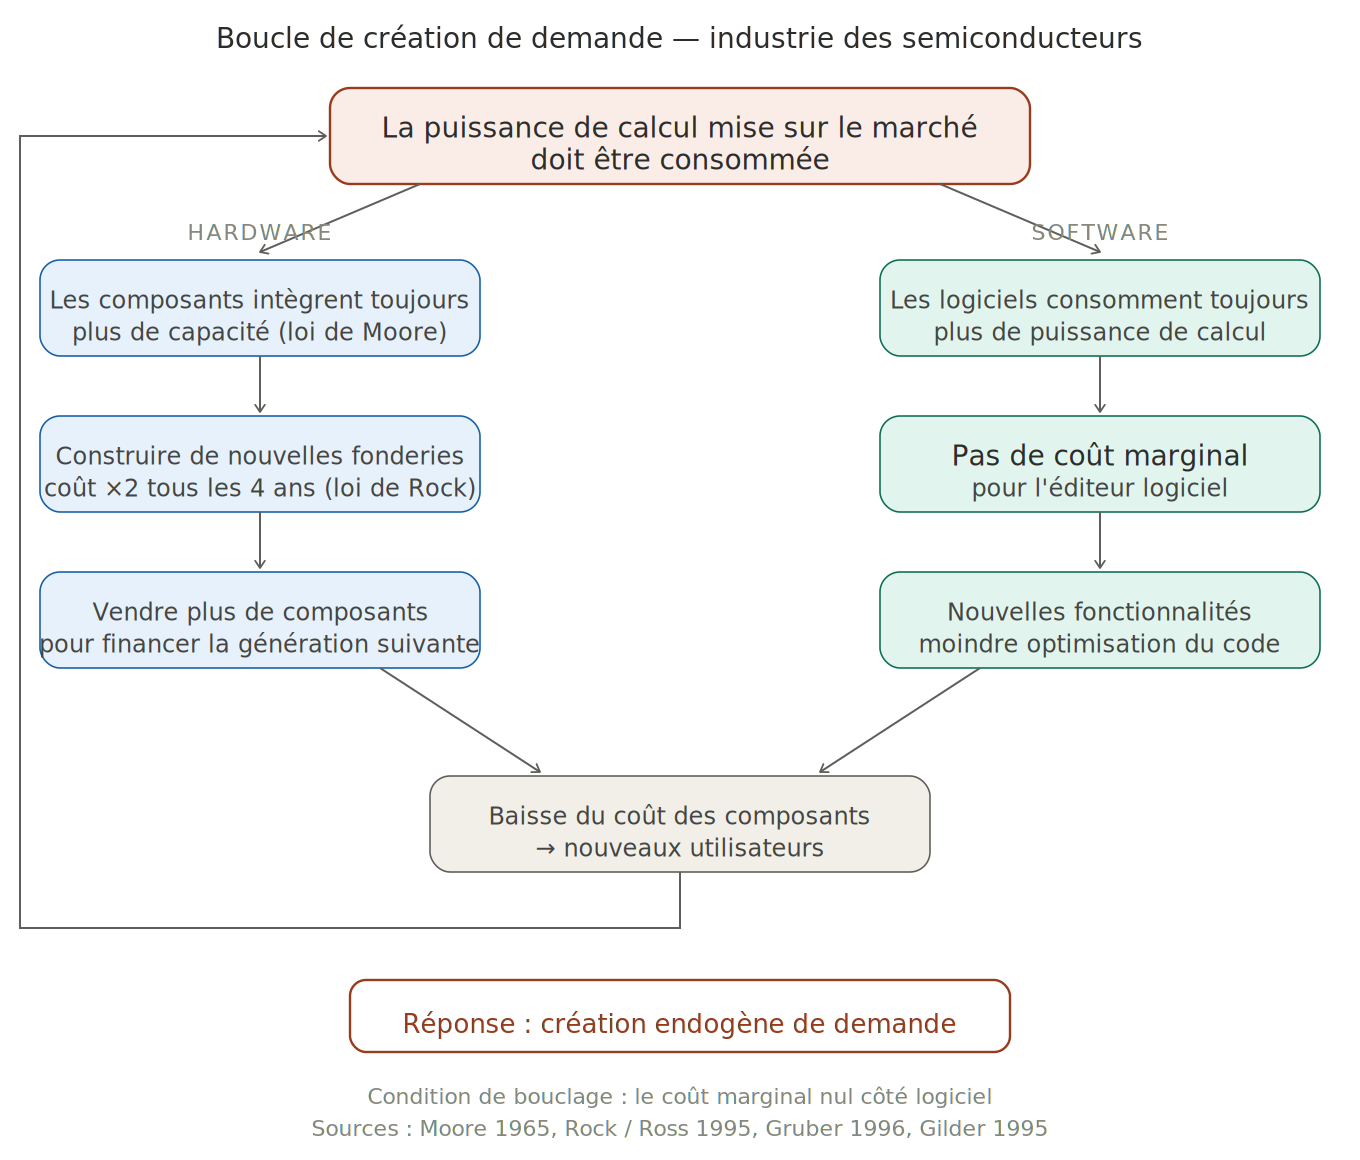
\includegraphics[width=0.92\textwidth]{Figures/fig1_semiconductor_demand_loop}
\caption{Boucle de création de demande dans l'industrie des semi-conducteurs. La contrainte d'investissement (Rock) force l'absorption du compute~; la coordination hardware-software (Wintel) fournit la soupape~; le coût marginal nul côté logiciel est la condition de bouclage. L'empreinte environnementale croît comme externalité, sans rétroaction sur la boucle.}
\label{fig:semicond-loop}
\end{figure}

Parallèlement, la loi de \textcite{dennard_design_1974} garantissait que la miniaturisation n'augmentait pas la densité de puissance électrique des composants~: plus de transistors sur la même surface, mais pas plus de chaleur. Ce mariage entre Moore et Dennard a tenu jusqu'aux alentours de 2005, lorsque la fréquence des processeurs a plafonné autour de 3~GHz \parencite{rupp_microprocessor_2018}. La réponse a été la multiplication des cœurs et l'essor du calcul parallèle~--- mais la rupture de Dennard a ouvert la voie à une trajectoire nouvelle~: l'augmentation de la puissance électrique par composant, longtemps contenue, est devenue une variable d'ajustement.

Une estimation exploratoire sur données françaises (comptes nationaux INSEE, 2000--2020) suggère que le capital numérique à destination productive concentre environ 97\,\% du stock total, une structure quasi constante sur vingt ans malgré les engagements climatiques successifs\footnote{Estimation du Papier~1 de la présente thèse, fondée sur un modèle de dynamique des systèmes calibré sur données INSEE, SDES et CITEPA.}.

\section{L'IA générative~: un changement de régime dans la consommation de puissance}

L'irruption de l'apprentissage profond sur GPU à partir de 2012 \parencite{krizhevsky_imagenet_2012} et l'accélération de l'IA générative depuis 2018 modifient plusieurs paramètres de cet équilibre.

Premièrement, les fournisseurs de modèles se trouvent dans la position qu'occupait Microsoft dans les années~1990~: ils doivent absorber la puissance de calcul mise sur le marché. Mais le rythme est différent. \textcite{openai_ai_2018} ont estimé que la demande de compute pour l'entraînement de modèles doublait tous les 3,4~mois entre 2012 et 2018~--- un rythme sans commune mesure avec celui de la loi de Moore. \textcite{kaplan_scaling_2020} ont formalisé cette dynamique en lois de puissance reliant la taille du modèle, la taille du jeu de données et le compute d'entraînement à la performance. Ces lois jouent un rôle performatif comparable à celui de Moore~: elles organisent la R\&D, structurent les feuilles de route et mobilisent les capitaux. \textcite{cahn_question_2024} a estimé à 600~milliards de dollars l'écart entre ce qui a été investi dans les entreprises d'IA générative et ce qu'elles ont généré en revenus.

Deuxièmement, l'inférence~--- la production d'un résultat par un modèle entraîné~--- a un coût marginal en énergie qui n'existait pas dans le logiciel traditionnel. Chaque token produit consomme de l'électricité. \textcite{cottier_rapid_2025} documentent une baisse médiane du coût d'inférence de l'ordre de $\div 50\times$ par an à performance fixe, mais le coût marginal reste structurellement positif~--- contrairement au logiciel classique. Les fournisseurs de modèles doivent donc simultanément maximiser l'adoption (pour absorber le compute) et minimiser le coût marginal (pour être rentables)~--- deux objectifs en tension. La figure~\ref{fig:genai-loops} rend visible cette structure~: une boucle de renforcement (profitabilité, utilisateurs, conversion) et une boucle de régulation (coût marginal par token) qui n'existait pas dans le modèle classique de la figure~\ref{fig:semicond-loop}.

\begin{figure}[htbp]
\centering
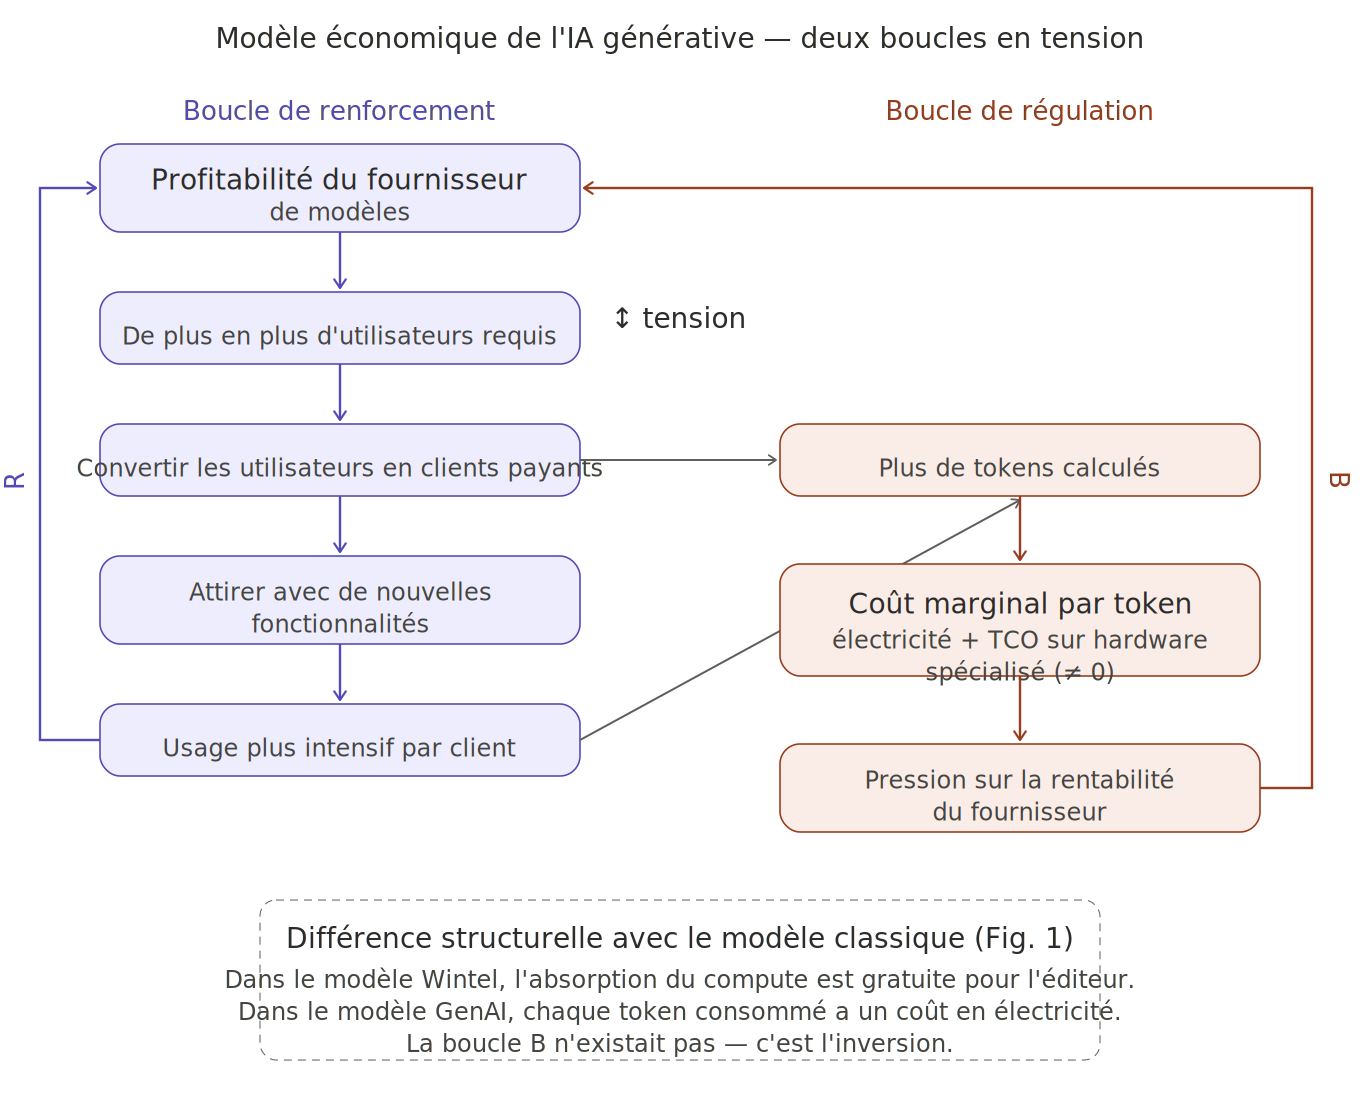
\includegraphics[width=0.92\textwidth]{Figures/fig2_genai_two_loops}
\caption{Modèle économique de l'IA générative~: deux boucles en tension. La boucle de renforcement (gauche) pousse à l'adoption massive~; la boucle de régulation (droite) introduit un coût marginal par token qui n'a pas d'équivalent dans le modèle Wintel. La tension entre les deux boucles est le fait structurel nouveau.}
\label{fig:genai-loops}
\end{figure}

Troisièmement, la puissance électrique des composants augmente de manière spectaculaire. Le TDP (\emph{Thermal Design Power}) des GPU est passé de 150~W (gamme stable 2005--2018) à des projections de 1\,400~W pour 2026--2027 selon les feuilles de route de Nvidia et AMD \parencite{sun_chip_2024}. L'empreinte environnementale par cm$^2$ de surface gravée, qui avait baissé depuis les années~1990, ré-augmente sous le seuil des 10~nm du fait des nouvelles contraintes de lithographie \parencite{pirson_environmental_2022}. \textcite{epoch_electricity_2025} projettent une demande électrique des centres de données IA supérieure à 30~GW aux États-Unis d'ici 2030, soit environ 5\,\% de la génération électrique totale.

Cette tension entre fabricants de hardware et fournisseurs de modèles produit une structure d'incitations divergentes que la figure~\ref{fig:tension-hw-models} schématise~: que l'efficacité de l'inférence progresse vite ou qu'elle stagne, les deux scénarios convergent vers des difficultés pour l'écosystème.

\begin{figure}[htbp]
\centering
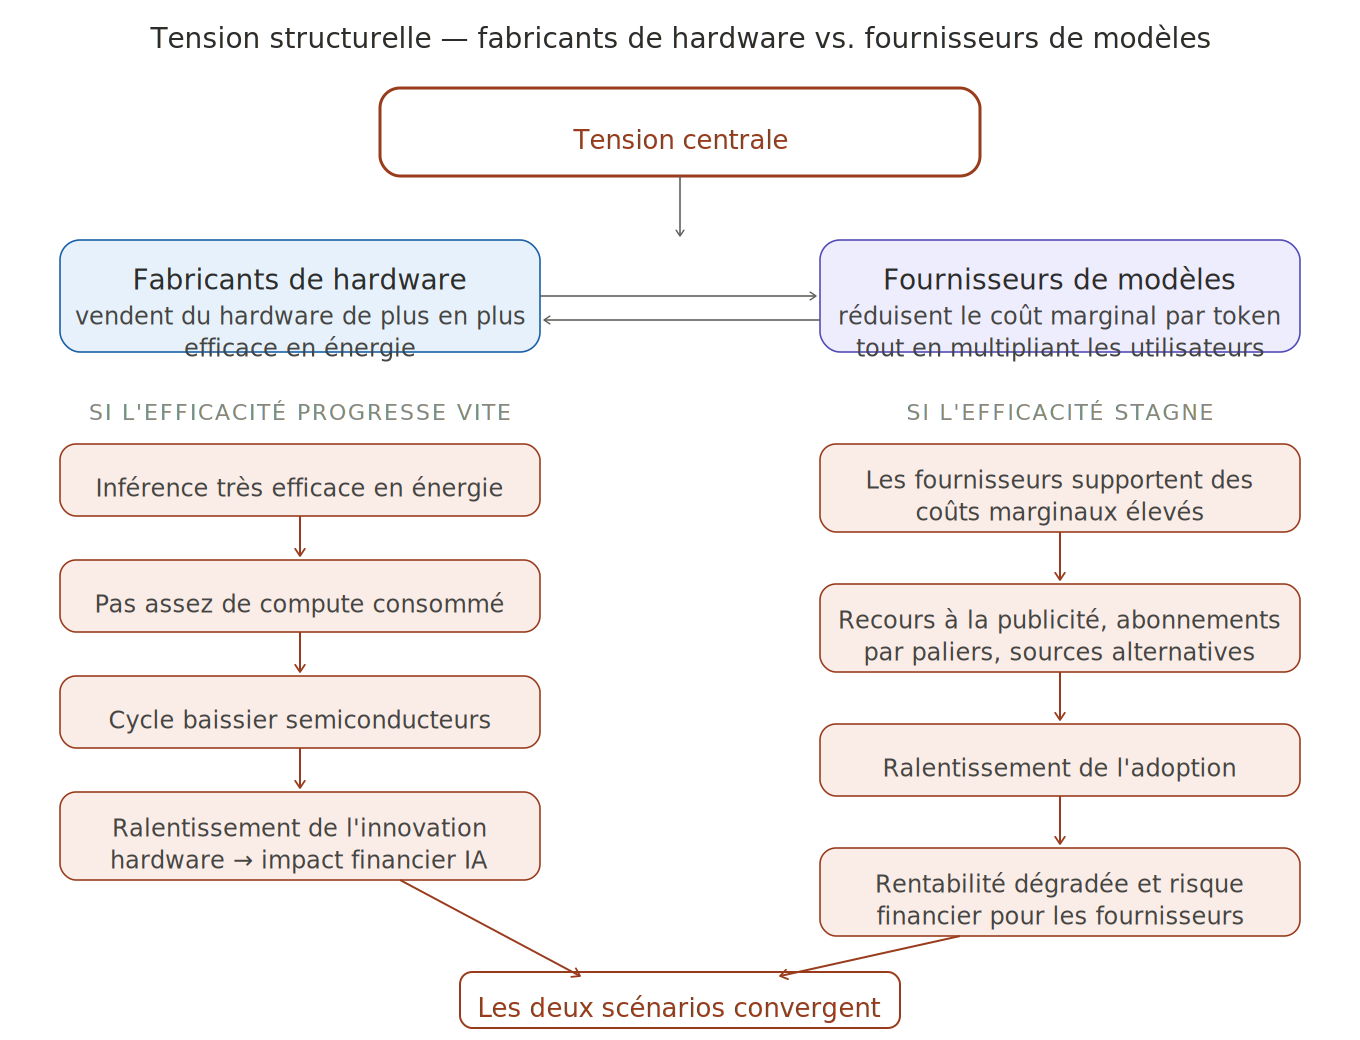
\includegraphics[width=0.92\textwidth]{Figures/fig5_tension_hardware_models}
\caption{Tension structurelle entre fabricants de hardware et fournisseurs de modèles. Les deux scénarios~--- efficacité rapide (gauche) et efficacité stagnante (droite)~--- convergent vers des difficultés financières pour l'écosystème. C'est une structure d'incitations divergentes qui n'a pas d'équivalent dans le cas télégraphe, où Western Union fabriquait, posait et exploitait le réseau.}
\label{fig:tension-hw-models}
\end{figure}

\section{Confrontation avec les mécanismes du chapitre~2}

Pour structurer la comparaison, la figure~\ref{fig:telegraph-cld} schématise les dynamiques structurelles du cas télégraphe telles qu'elles émergent du chapitre~1~: deux boucles de renforcement (la création de marchés par l'information synchrone et la coordination des systèmes physiques complexes) et une propriété transversale~--- la boucle ouverte côté énergie. Mise en regard des figures~\ref{fig:semicond-loop}, \ref{fig:genai-loops} et~\ref{fig:tension-hw-models}, elle rend visible les continuités et les ruptures.

\begin{figure}[htbp]
\centering
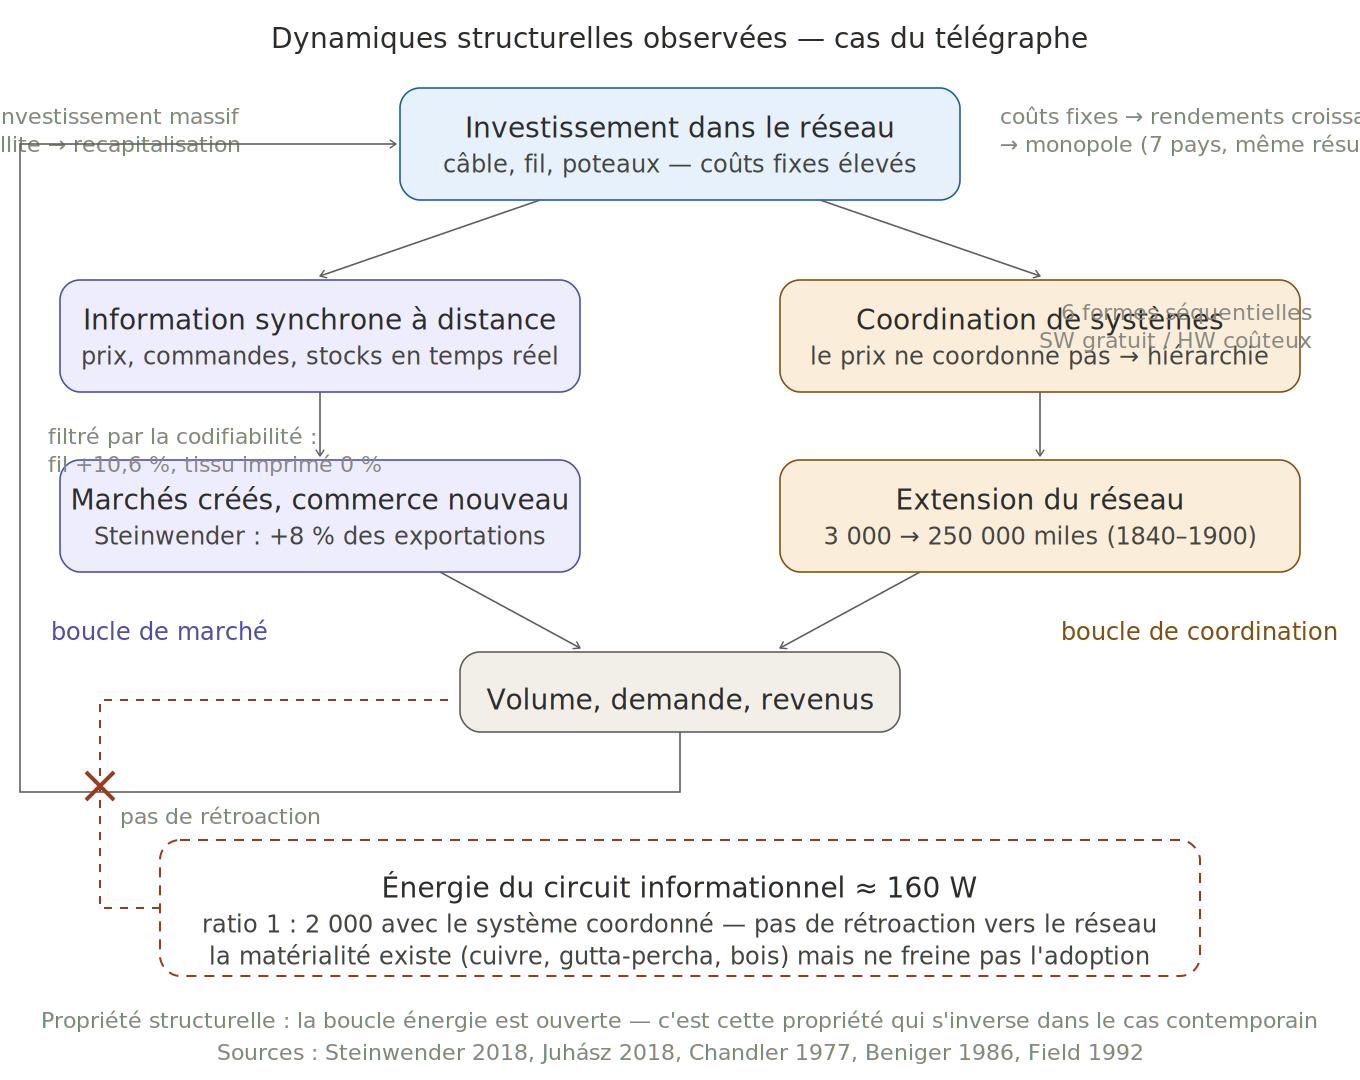
\includegraphics[width=0.92\textwidth]{Figures/fig_telegraph_structural_dynamics}
\caption{Dynamiques structurelles du cas télégraphe (synthèse du chapitre~1). Deux boucles de renforcement~--- la création de marchés (Steinwender) et la coordination ferroviaire (Chandler, Beniger)~--- alimentent l'investissement. La propriété structurelle centrale est la boucle ouverte énergie~: le coût énergétique du circuit informationnel ($\approx$~160~W) est négligeable face au système coordonné (ratio 1:2\,000), ce qui supprime toute rétroaction. C'est cette propriété qui s'inverse dans le cas contemporain.}
\label{fig:telegraph-cld}
\end{figure}

Le tableau~\ref{tab:dim-telegraph-genai} concentre la confrontation sur les six dimensions où le matériau empirique est le plus substantiel. La colonne de gauche synthétise les résultats du chapitre~1~; la colonne de droite mêle deux objets distincts~--- l'industrie des semi-conducteurs et l'IA générative~--- dont la fragmentation même (modèle \emph{fabless/foundry}, séparation entre conception, gravure et usage) est un fait structurel sans équivalent dans le cas télégraphe. Trois catégories de diagnostic sont distinguées~: un mécanisme est dit \emph{invariant} lorsque la même structure causale opère dans les deux cas~; en \emph{accélération} lorsque le rythme s'accroît~; en \emph{inversion} lorsque la direction change de signe.

\begin{table}[p]
\caption{Du télégraphe à l'infrastructure de calcul~: six dimensions substantielles}\label{tab:dim-telegraph-genai}
\centering\footnotesize
\renewcommand{\arraystretch}{1.15}
\begin{tabularx}{\textwidth}{@{}cp{2.8cm}p{3.3cm}cp{4.2cm}@{}}
\toprule
 & \textbf{Télégraphe (synthèse ch.~1)} & \textbf{Infrastructure de calcul et IA générative} & \textbf{Verdict} & \textbf{Ce qui explique l'écart} \\
\midrule
D1 & Signal rival, information non rivale (câble, Chappe) & Output non rival, inputs rivaux (interface~: le training consomme le compute produit) \parencite{cottier_rapid_2025} & Inversion & Coût marginal de l'usage redevient positif. Rapport rival/non-rival s'inverse côté production. \\[3pt]
D2 & Coûts fixes $\rightarrow$ 7~modèles $\rightarrow$ monopole (7~pays) & Loi de Rock $\rightarrow$ concentration TSMC/Samsung (semi-cond.). Oligopole cloud (GenAI) \parencite{gruber_semiconductor_1996} & Invariant & Même mécanisme, seule l'échelle change. \\[3pt]
D3 & Capital linéaire, durée de vie $\sim$10~ans. K/L universelle (4~pays) & GPU obsolète en 18--24 mois (semi-cond.). Temporalités croisées bâtiment/GPU/modèle/PPA (cf.~section~\ref{sec:d3-capital}) & Accélération & Dépréciation comprimée. Le gradient isolé/intégré du ch.~2 s'applique. \\[3pt]
D5 & Prix au mot. Baisse $\rightarrow$ explosion du volume (US, FR) & Coût/token $\neq$ 0 (GenAI). Gaspillage nécessaire pour absorber le compute (interface) \parencite{cottier_rapid_2025} & Inversion & Le gaspillage avait coût nul pour l'éditeur. L'inférence a un prix. \\[3pt]
D8 & Câble transatl.~: investissement $\rightarrow$ faillite $\rightarrow$ recap. & 600~Md\$ de gap (GenAI) \parencite{cahn_question_2024}. Scaling laws performatives (interface) \parencite{kaplan_scaling_2020}. Cyclicité WSTS (semi-cond.) & Invariant & Même enchaînement. Performativité plus explicite. \\[3pt]
\midrule
0-TER & Boucle ouverte~: ratio circuit informationnel/énergie $\approx$ 1:2\,000, pas de rétroaction (cas ferroviaire) & Boucle se fermant~: TDP 150 $\rightarrow$ 1\,400~W (semi-cond.). Datacenters $>$30~GW (interface) \parencite{epoch_electricity_2025}. Coût élec./token (GenAI) & Inversion & Le coût énergétique de l'information franchit le seuil de visibilité macro~: la boucle se ferme. \\
\bottomrule
\end{tabularx}
\renewcommand{\arraystretch}{1.0}
\end{table}

Quatre autres dimensions sont touchées par le cas semi-conducteurs/IA, mais avec un matériau moins propre à cette annexe qu'aux sections correspondantes du chapitre~2. L'automatisation du travail cognitif (dimension~4) est un fait documenté \parencite{acemoglu_simple_2024}, mais le mécanisme est générique~--- il ne dépend pas spécifiquement de l'infrastructure de calcul. L'opacification possible du signal de prix par la tarification algorithmique (dimension~6) reste une hypothèse ouverte sans documentation économétrique comparable à celle de \textcite{steinwender_real_2018} pour le télégraphe. La ré-intégration verticale des hyperscalers~--- puces propriétaires (Google TPU, Amazon Graviton), contrats d'énergie directs~--- pose la question de la frontière firme-marché (dimension~7), mais sans traitement analytique suffisant pour un verdict. La géographie de la chaîne de valeur GPU~--- concentration de la gravure à Taiwan, embargos américains \parencite{miller_chip_2022}~--- et le verrouillage de trajectoire technologique (dimensions~9 et~10) sont les cas contemporains les plus documentés de concentration géographique de l'infrastructure informationnelle~; ils sont traités dans les sections correspondantes du chapitre~2.

\section{Le couplage~: décomposition et explicitation}

Le résultat principal du tableau n'est pas qu'une dimension nouvelle émerge~--- aucune n'émerge. Le cadre analytique construit à partir du cas télégraphe capture l'intégralité des mécanismes observés dans le cas contemporain. Le résultat est ailleurs~: dans la simultanéité de quatre inversions qui, en se produisant en même temps, font apparaître le couplage entre infrastructure informationnelle et substrat énergétique là où il était masqué.

La première inversion concerne la composition du bien informationnel (D1). La production de biens non rivaux~--- les modèles entraînés, dont le coût marginal de reproduction tend vers zéro~--- est devenue massivement rivale en inputs~: le compute d'entraînement des modèles frontier consomme plus de 100~MW pendant des semaines \parencite{epoch_electricity_2025}, et l'inférence acquiert un coût marginal en énergie par token qui n'existait pas dans le logiciel traditionnel \parencite{cottier_rapid_2025}. Le rapport entre la couche non rivale et la couche rivale du bien composite, tel qu'il est analysé dans la dimension D1, s'inverse côté production.

La deuxième inversion concerne la demande et les coûts marginaux (D5). Pendant quatre décennies, l'industrie du logiciel a pu absorber les gains de puissance sans coût marginal~: utiliser davantage de transistors ne coûtait rien à l'éditeur \parencite{gilder_coming_1995, schaller_origin_1996}. L'inférence de l'IA générative rompt cette gratuité. Le gaspillage de puissance~--- qui était le mécanisme même de soutien aux économies d'échelle de l'industrie des semi-conducteurs~--- a désormais un prix pour le fournisseur de modèle. Il en résulte une tension structurelle~: l'industrie des semi-conducteurs a besoin que le compute soit consommé (D2), mais le consommer coûte de l'énergie (0-TER), et ce coût grève la rentabilité du fournisseur (D5).

La troisième inversion, plus spéculative, concerne le signal de prix (D6). Le télégraphe améliorait la transparence des marchés~: il synchronisait les prix, réduisait les asymétries, créait des marchés unifiés \parencite{steinwender_real_2018}. L'IA compute-intensive pourrait, à l'inverse, opacifier le signal de prix par la tarification algorithmique, la personnalisation et l'asymétrie computationnelle entre offreur et demandeur. Ce diagnostic reste une hypothèse ouverte~: il n'existe pas, à notre connaissance, d'étude économétrique comparable à celle de \textcite{steinwender_real_2018} qui documenterait l'effet de l'IA sur la transparence des marchés.

La quatrième inversion, empiriquement la plus robuste, concerne le couplage énergétique (0-TER). Le ratio entre la puissance du circuit informationnel et la puissance du système qu'il coordonne, de l'ordre de 1:2\,000 pour le télégraphe ferroviaire du dix-neuvième siècle, franchit le seuil de visibilité macroéconomique lorsque les centres de données IA projettent une demande supérieure à 30~GW, soit plusieurs pourcents de la génération électrique américaine \parencite{epoch_electricity_2025, iea_data_2024}. Le TDP des composants, longtemps stabilisé entre 75 et 150~W, atteint 1\,200~W (Nvidia GB200) et vise 1\,400~W à l'horizon 2027 \parencite{sun_chip_2024}. L'empreinte de fabrication par cm$^2$, qui avait diminué jusqu'au seuil des 10~nm, ré-augmente pour les nœuds avancés \parencite{pirson_environmental_2022}.

C'est la simultanéité de ces inversions qui constitue le phénomène~: le couplage entre l'infrastructure informationnelle et le substrat énergétique, qui avait toujours existé mais était analytiquement invisible parce que les ordres de grandeur le rendaient négligeable, devient un fait macroéconomique structurant. Les dimensions qui étaient jusqu'alors séparables~--- parce que le coût énergétique de l'ICT pouvait être ignoré~--- cessent de l'être. L'industrie des semi-conducteurs doit désormais traiter l'énergie comme une variable de premier ordre \parencite{epoch_electricity_2025}~; les fournisseurs de modèles signent des contrats d'achat d'électricité (\emph{PPA}) directement avec des centrales~; les centres de données deviennent des acteurs du système électrique, pas seulement des consommateurs passifs.

Ce couplage pourrait ne pas être un phénomène contingent~--- pas un accident de la phase actuelle de l'IA~--- mais une conséquence de l'évolution des dimensions qui s'inversent. Si la production de non-rivalité est rivale en énergie (D1), si l'absorption du compute a un coût marginal (D5), si la puissance électrique des composants croît au lieu de stagner (0-TER), alors le couplage entre information et énergie pourrait être structurel plutôt qu'accidentel~--- mais cette hypothèse reste à instruire. C'est ce couplage~--- sa décomposition en dimensions, son explicitation en mécanismes, sa quantification éventuelle dans un cadre de modélisation macroéconomique~--- qui constitue la question centrale de cette thèse.

\section{Limites et statut du diagnostic}

Ce diagnostic est une première exploration, pas un résultat. Les deux verdicts \og invariant\fg{} (D2 et D8) sont les plus solides~: la concentration vers le monopole \parencite{gruber_semiconductor_1996} et les cycles d'investissement \parencite{perez_technological_2002} sont documentés indépendamment dans les deux cas par des littératures distinctes. L'accélération de D3 est étayée par les données de dépréciation des GPU et par le gradient isolé/intégré développé à la section~\ref{sec:d3-capital} du chapitre~2. Parmi les inversions, celle de 0-TER est empiriquement la plus robuste (données IEA, EPRI, Epoch), celle de D1 est étayée par les données de \textcite{cottier_rapid_2025} et \textcite{epoch_electricity_2025}, celle de D5 est un fait observable (le coût par token est documenté et publié). L'inversion de D6, discutée dans la section~4, est spéculative et devrait être traitée comme une hypothèse à instruire, pas comme un acquis. Les dimensions traitées en prose (D4, D7, D9, D10) sont des analogies structurelles plausibles mais non testées causalement dans le cadre de cette annexe~: elles relèvent du traitement systématique du chapitre~2.

Le terme de \emph{couplage}~--- ou plus précisément de \emph{re-couplage}, puisque le lien entre information et énergie a toujours existé mais était masqué~--- est proposé pour désigner ce que les inversions simultanées révèlent~: le moment où l'infrastructure informationnelle redevient suffisamment matérielle pour que les économistes de l'énergie et les économistes de l'information ne puissent plus s'ignorer.
